\section{Learning with SGD}
\frame{\tableofcontents[currentsection, hideothersubsections]}

\begin{frame}
\frametitle{SGD for Risk Minimization}

Recall, in learning:\\
\begin{itemize}
\item want to minimize the risk function, $L_D(w) = \mathbb{E}_{z \approx D} [l(w, z)]$
\item do not know $D$, so cannot simply calculate $LD (w(t))$
\end{itemize}

With SGD:\\
find an unbiased estimate of the gradient of $L_D(w)$, that is,
a random vector whose conditional expected value is $LD (w(t) )$

\end{frame}


\begin{frame}
\frametitle{SGD for Risk Minimization}

Consider a differentiable risk function $L_D$.

The construction of the random vector $v_t$:
\begin{itemize}
\item sample $z \approx D$
\item define $v_t$ to be the gradient of the function $l(w, z)$ wrt $w$, at $w^{(t)}$
\item by the linearity of the gradient we have:
\end{itemize}

% Thus, the gradient of the loss function `(w, z) at w (t) is
% \item unbiased estimate of the gradient of the risk function LD (w (t) ) and
% \item is easily constructed by sampling a single fresh example z ∼ D at each iteration t.

\end{frame}


\begin{frame}
\frametitle{SGD for Risk Minimization}

\begin{figure}
    \centering
    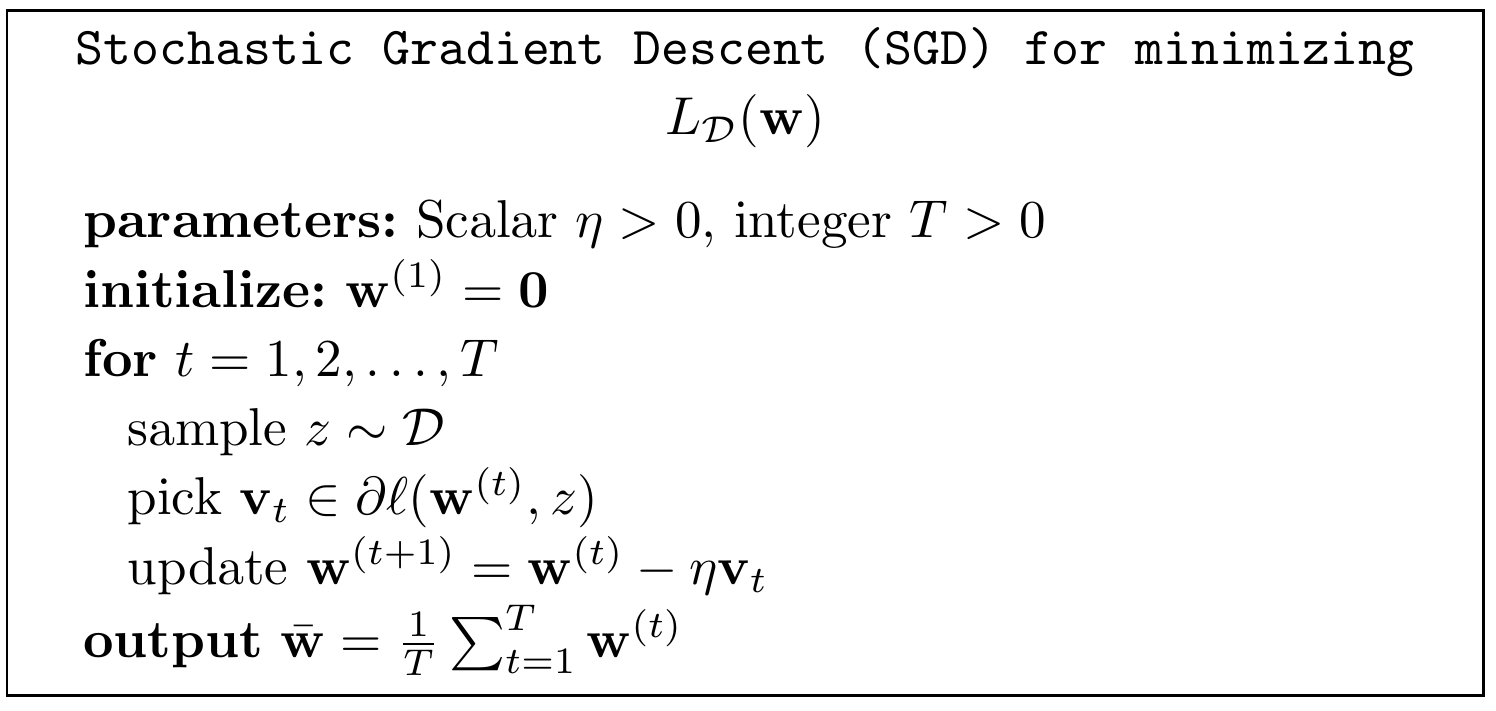
\includegraphics[scale=0.25]{sgd2}
\end{figure}

\end{frame}
